%------------------------------------------------------------------------
%Editar Diplomado
\hypertarget{cv:registrarProyectoAdmin}{\section{Registrar Proyecto de Administrador}} \label{sec:registrarProyectoAdmin}

	Esta funcionalidad le permitirá registrar la información general de un proyecto en el sistema, dichos datos se guardan con el objetivo de conocer las propiedades referentes a cada proyecto, 

		\subsection{Procedimiento}

			%Pasos de procedimiento
			\begin{enumerate}
	
			\item Oprima el botón \IURegistrar{} de la pantalla \ref{fig:GestionarProyectosAdmin} ''Gestionar Proyectos de Administrador''.
			
			\item Se mostrará la pantalla \ref{fig:registrarProyecto} ''Registrar Proyecto''.

			%Pantalla
			\begin{figure}[htbp!]
				\begin{center}
					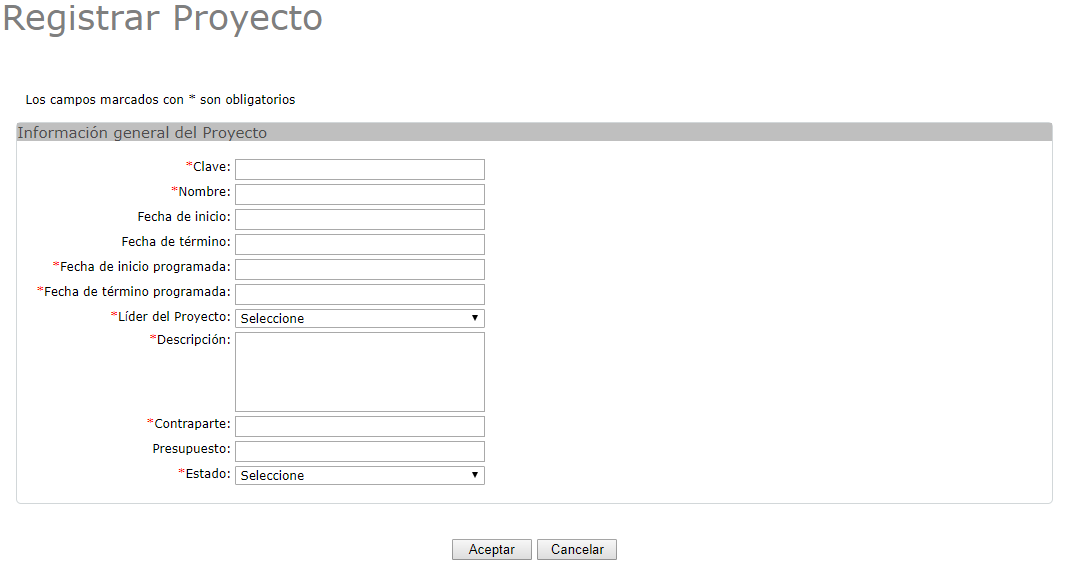
\includegraphics[scale=0.6]{roles/administrador/proyectosAdmin/gestionarproyectosAdmin/pantallas/IU2-1registrarProyecto}
					\caption{Registrar Proyecto de Administrador}
					\label{fig:registrarProyecto}
				\end{center}
			\end{figure}
		
			\item Ingrese los datos correspondientes a la información  de un proyecto como su clave, nombre, las fechas de inicio y término del mismo. También es necesario que se asigne un líder de proyecto, una descripción, la contraparte que solicita el proyecto y que estado se le asignará al proyecto. Si lo desea puede ingresar el presupuesto con el que se cuenta para iniciar el proyecto.
			
			\item Oprima el botón \IUAceptar.
			
			\item Se mostrará el mensaje \ref{fig:proyectoRegistrado} en la pantalla \ref{fig:GestionarProyectosAdmin} ''Gestionar Proyectos de Administrador''.
			
			\begin{figure}[htbp!]
				\begin{center}
					
\includegraphics[scale=0.6]{roles/administrador/proyectosAdmin/gestionarproyectosAdmin/pantallas/IU2-1MSG1}
					\caption{MSG: Proyecto Registrado}
					\label{fig:proyectoRegistrado}
				\end{center}
			\end{figure}
			\end{enumerate}